\chapter{Introduction To Finance}


\section{The purpose of a corporation}

\begin{definitionbox}{Definition of a Corporation}
    \begin{itemize}
    \item A legal entity distinct from its owners, known as \textbf{shareholders}.
    \item Created upon filing legal documents with government
    \item It is conferred some legal rights and privileges e.g. limited liability, but also legal obligations, e.g. paying tax.
\begin{itemize}
        \item Limited liability: shareholder's personal assets are protected even thought the corporation faces financial difficulties
        \item Shareholders are only liable for amount invested
        \item Corporations can exist indefinitely despite ownership/management changes, allowing them to pursue long-term strategies to increase value
        \item Can raise capital through issuance of stocks and bonds, allowing them to access funding from investors to finance growth  
\end{itemize}
    \item Goal: maximise shareholder's investments over time
\end{itemize}
\end{definitionbox}

\subsection*{Considering Stakeholders}
Corporations are generally viewed as drivers to maximise shareholder value, but there has been a growing recognition of the importance of considering other people who are directly or indirectly affected by the externalities of a corporation, the \textbf{stakeholders}. 

Examples of stakeholders:
\begin{itemize}
    \item Customers
    \item Employees
    \item Suppliers
\end{itemize}

Focusing on their interests could lead to possible benefits such as increased customer loyalty, employee satisfaction, and supplier reliability.

It is important to strike a balance between the interests of shareholders and stakeholders, as the focusing too much on stakeholders' interests could dilute the primary goal of maximising shareholder value.


\section{Financial Intermediation}

\subsection*{Definition}
Financial intermediation refers to the process of transferring funds from those who have excess funds to those who need funds.

\subsection*{Simplified Model}
Consider a simplified modern economy with two key players: the household sector (representing individuals wishing to save for various purposes such as retirement), and the business sector (representing firms that require funds to finance their operations).

\begin{itemize}
    \item Households save by depositing funds in banks, which in turn lend these funds to businesses. \textbf{The bank serves as the financial intermediary.}
    \item While it's theoretically possible for households to lend directly to businesses, this would incur large transaction costs, so banks make the process more efficient.
    \item Businesses use these funds to finance their operations, and in return, pay interest to the banks. 
    \item Banks earn a profit by charging a higher interest rate on loans than the interest rate paid on deposits.
\end{itemize}

There are three types of transformations on the flow of capital:
\begin{enumerate}
    \item Size Transformation:
    \begin{itemize}
        \item Savers can lend small amounts, banks will pool these funds to make large loans to businesses.
    \end{itemize}
    \item Maturity Transformation:
    \begin{itemize}
        \item Borrowing short and lending long: Banks allow savers to withdraw or deposit funds at any time, offering liquidity to savers, but can lend to businesses for longer periods.
        \item This works as long as the amount of money savers want to withdraw is offset by the amount savers are putting in. 
        \item Problems can occur if there is a sudden rush of withdrawals, leading to a bank run, where a bank runs out of cash to meet withdrawal demands. It cannot call in its loans to businesses to meet these demands, as they are long-term and illiquid.
    \end{itemize}
    \item Risk Transformation:
    \begin{itemize}
        \item Savers indirectly invest in many small projects spreading their risk, but borrowers can invest their whole loan in one project.
    \end{itemize}
\end{enumerate}

\begin{figure}[H]
    \centering
    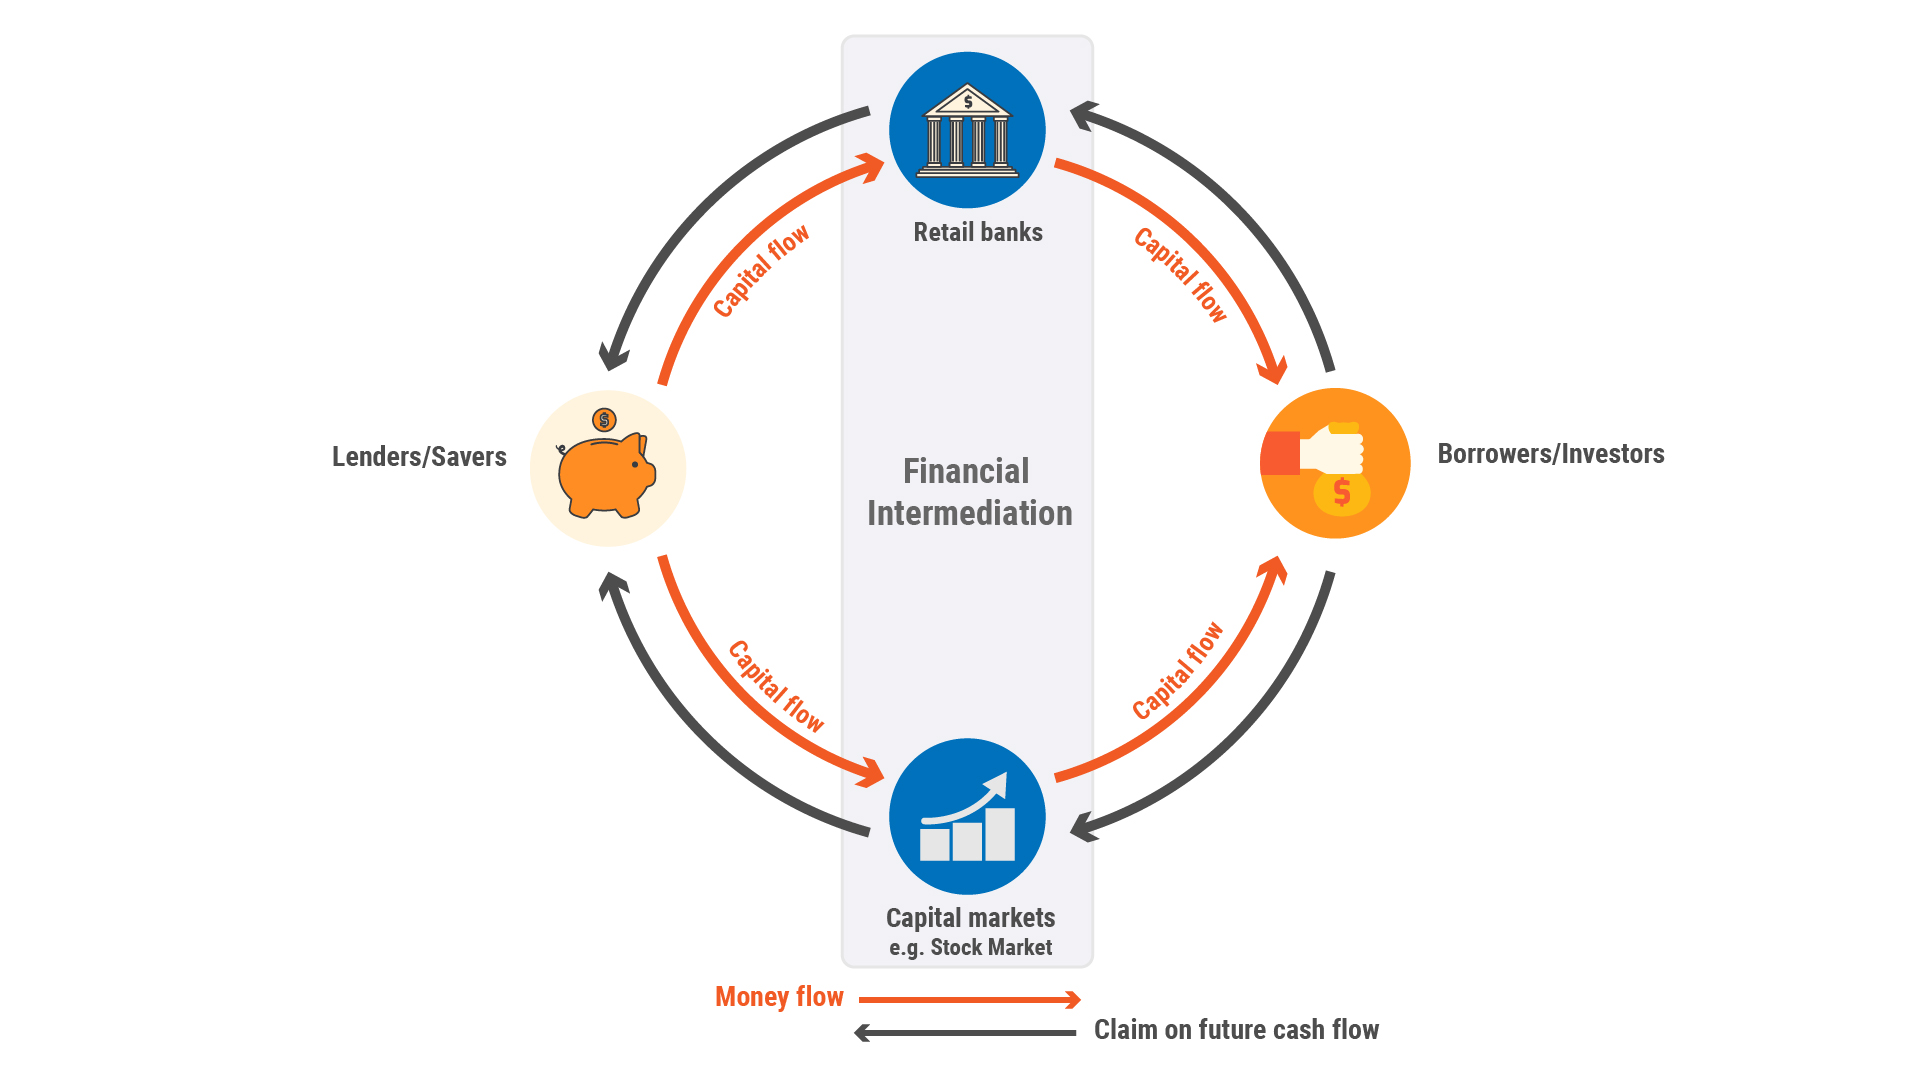
\includegraphics[width=0.8\textwidth]{img/1.1.jpeg}
    \caption{Financial Intermediation}
    \label{fig:financial_intermediation}
\end{figure}

\section{Basic Securities}

A business can raise money to fund their investment projects through borrowing from the bank as a loan. They can also sell debt securities, or bonds, to investors. Similar to a loan, the firm agrees to make regular interest payments over the loan's term and repay the loan in full at the end.

A loan can also raise funds through public markets by selling equity securities, or stocks, to investors. In return, investors receive a share of the firm's profits in the form of dividends, and the potential for capital gains if the stock price increases. Shares grant the buyer s take in the ownership of the company, and the right to vote on company decisions.

\subsection*{Main Institutions in Financial Markets}

\begin{enumerate}
    \item \textbf{Buy-side:}
    \begin{itemize}[noitemsep]
        \item Dominated by asset managers and insurance companies like AIG.
        \item Examples include Prudential, Aviva, and mutual fund managers like BlackRock.
        \item Notable hedge funds include Citadel and Bridgewater Associates.
        \item Large corporations manage substantial pension funds, e.g., Shell and General Motors.
    \end{itemize}
    
    \item \textbf{Sell-side:}
    \begin{itemize}[noitemsep]
        \item Involves major universal banks (e.g., UBS, Bank of America) and specialised investment banks (e.g., J.P. Morgan, Goldman Sachs).
        \item These institutions offer brokerage services and engage in buy-side activities.
    \end{itemize}
\end{enumerate}


\begin{table}[htbp]
    \centering
    \caption{Differences between Debt and Equity}
    \label{tab:debt-equity}
    \begin{tabular}{@{}>{\raggedright}p{2.5cm}>{\raggedright\arraybackslash}p{5.5cm}>{\raggedright\arraybackslash}p{5.5cm}@{}}
    \toprule
     & \textbf{Debt} & \textbf{Equity} \\ \midrule
    \textbf{Ownership} & Not an ownership interest. Creditors do not have voting rights. & Ownership interest. Common stockholders vote on board of directors and other issues. \\
    \textbf{Tax} & Interest is considered a cost of doing business and is tax-deductible. & Dividends are not considered a cost of doing business and are not tax-deductible. \\
    \textbf{Longevity} & Debt has a specific term after which capital must be repaid or rolled over. & Equity is infinitely lived, so capital is effectively loaned in perpetuity. \\
    \textbf{Return risk} & Under normal circumstances, debt holders know cash flows in advance. & Equity holders receive a share of profits which is unknown in advance. \\
    \textbf{Credit risk} & Creditors have legal recourse if interest or principal payments are missed. & Dividends are not a liability of the firm and stockholders have no legal recourse if no dividends are paid. \\
    \bottomrule
    \end{tabular}

\end{table}


    
\section{Financial Crises}
2007 was the start of the Global Financial Crisis, which was caused by the collapse of the US housing market. 


Low interest rates post-9/11 meant there was a lot of borrowing and investment in housing, leading to a housing price bubble. \\

The crisis was triggered by the subprime mortgage crisis, where banks were lending to high-risk borrowers who could not afford to repay their loans. The crisis led to a global recession, with many banks and financial institutions collapsing and governments having to bail them out. \\

  
\textbf{Response and Reflection} (Discussion with Prof. Franklin Allen):
\begin{itemize}
    \item Regulators and central banks missed early signs due to a historic underestimation of widespread property price falls. Historically, the last nationwide decline in property prices was during the Great Depression, so central banks considered this very unlikely. 
    \item This resulted in failure to recognise increasing risks in the market.
    \item The crisis was similar to previous ones where asset bubbles led to banking issues that spilled over into the economy. Banks faced losses and were unable to lend (credit tightening), affecting broader economic growth.
    \item Current economic theories and models at central banks (which assume total market efficiency) failed to account for financial sectors in detail, and the dynamics of asset price bubbles which could disrupt the economy. So systemic risks by imbalances in the financial market were ignored.
\end{itemize}




